%\section{Hardware Architecture}
%Piattaforme aeree dei 2 droni, schede che usano, sensori usati
%\section{Software Framework}
%ROS2, integrazione con PX4,NODI PRINCIPALI COSA FANNO E CHE MESSAGGI SI SCAMBIANO, uso del bridge Micro-XRCE-DDS e modlaità offboard PX4

%\section{Optimization solver}
%DESCRIZIONE DI ACADOS E DELLE IMPOSTAZIONI DEL SOLVER USATE

This chapter details the practical implementation of the proposed cooperative aerial inspection framework. Translating the mathematical control formulation and shared control strategy into a functioning system requires a robust and real-time capable software architecture. The chapter discusses the middleware integration, the mission supervision layer, the real-time implementation of the observer drone's Non-linear Model Predictive Control (NMPC), the contact admittance filter for the inspection drone, and the haptic interface pipeline.
\section{Simulation and Hardware Setup}
The proposed framework is evaluated in both simulated and real-world environments. To ensure consistency between testing phases, the hardware and software architectures are designed to minimize the transition gap.
\\In the simulation environment, the robotic team is composed of two identical x500 quadrotor frames. The first vehicle, functioning as the Observer Drone, is equipped with a rigidly mounted virtual camera to stream the exocentric view. The second vehicle, the Inspection Drone, has a rigid link acting as an end-effector, featuring a 1D force sensor at its tip to measure environmental interaction forces during the contact task.
\begin{figure}[htbp]
    \centering
    \begin{subfigure}{0.49\textwidth}
        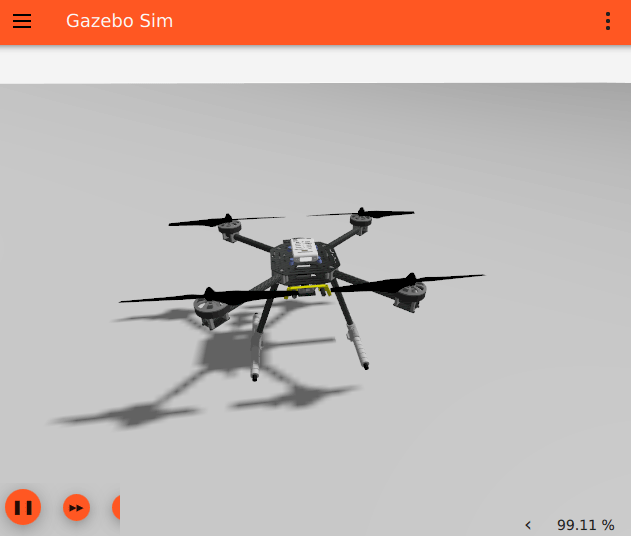
\includegraphics[width=\linewidth]{Immagini/Capitolo5/x500.DphTqKxq.png}    
    \end{subfigure}
    \begin{subfigure}{0.49\textwidth}
        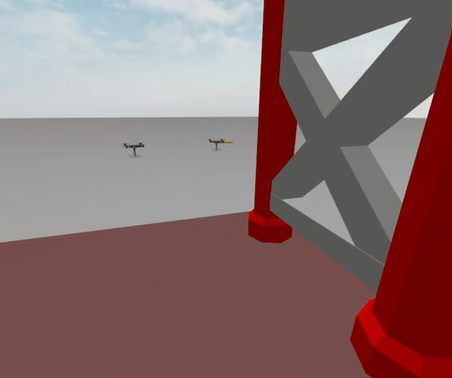
\includegraphics[width=\linewidth]{Immagini/Capitolo5/two_drones_one_bridge_2.png}    
    \end{subfigure}    
    \caption{Drones used in \texttt{SITL} simulation: x500 quadrotors - GazeboSim}
    \label{fig:placeholder}
\end{figure}
For the real-world experiments, the hardware implementation focuses entirely on validating the Observer Drone's optimal visual tracking and the associated haptic shared control. The physical Observer Drone is a custom-built octopter platform in flat configuration (whose model is mathematically equivalent to the quadrotor's one). Low-level attitude stabilization, motor mixing, and state estimation are handled by a Pixhawk flight controller. All high-level computations, including the ROS 2 middleware network, the NMPC solver, and the finite state machine, are executed onboard by a LattePanda companion computer connected to the flight controller via a serial interface.
\begin{figure}[htbp]
    \centering
    \begin{subfigure}{0.49\textwidth}
        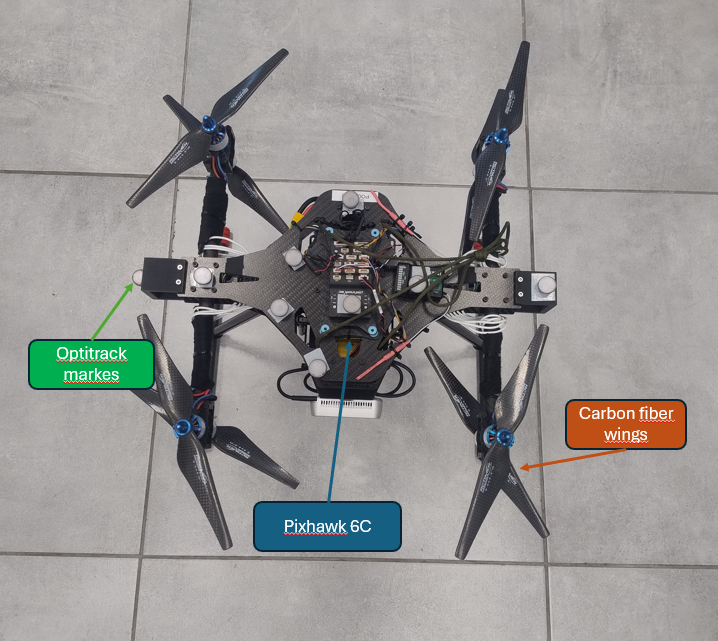
\includegraphics[width=\linewidth]{Immagini/Capitolo5/guardrone_up_labels.png}
    \label{fig:placeholder}
    \end{subfigure}
    \centering
    \begin{subfigure}{0.49\textwidth}
        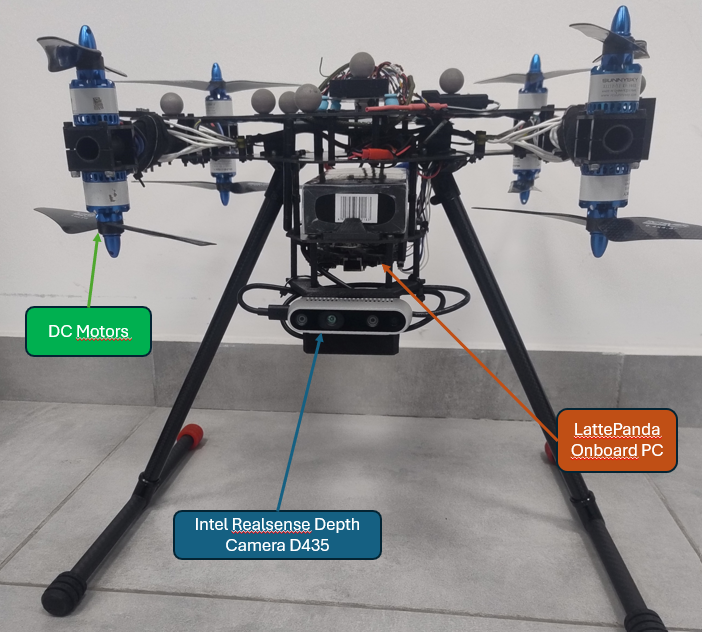
\includegraphics[width=\linewidth]{Immagini/Capitolo5/guardrone_front_labels.png}
    \label{fig:placeholder}
    \end{subfigure}
    \caption{Top and front views of real custom octocopter named \texttt{Pocho}, used for Observer UAV}
\end{figure}
Due to technical hardware constraints, the physical Inspection Drone is substituted by a manually piloted DJI quadrotor. This manually driven vehicle acts strictly as a dynamic physical target. This setup effectively tests the robustness of the observer's NMPC tracking capabilities and the human operator's haptic override in a dynamic scenario.
\section{Middleware and Simulation Architecture}
The high-level control network is developed within the Robot Operating System 2 (ROS 2) environment. ROS 2 provides a modular and distributed node architecture and relies on the Data Distribution Service (DDS) standard, ensuring the low-latency inter-process communication required for real-time control loops.
\\To interface the high-level ROS 2 network with the low-level hardware, the standard \texttt{PX4} open-source flight stack is utilized. Communication between the onboard LattePanda PC and the \texttt{Pixhawk} flight controller is handled by the \textit{Micro-XRCE-DDS} agent. This bridge directly maps the internal PX4 uORB messaging topics to ROS 2 DDS topics, allowing the control nodes to publish setpoints and read telemetry at high frequencies without custom serial protocols.
\begin{figure}[htpb]
    \centering
    \resizebox{\textwidth}{!}{% Ridimensiona in automatico ai margini della pagina
    \begin{tikzpicture}[
        >=stealth,
        node distance=1.5cm and 2cm,
        box/.style={rectangle, draw=black, thick, rounded corners, align=center, minimum height=1.2cm, minimum width=2.8cm, font=\small\sffamily},
        rosbox/.style={box, fill=blue!10},
        px4box/.style={box, fill=orange!10},
        envbox/.style={box, fill=green!10},
        devbox/.style={box, fill=gray!20},
        bridge/.style={rectangle, draw=black, thick, dashed, fill=gray!10, minimum height=9.5cm, minimum width=1cm, align=center,yshift=0.6cm, font=\small\sffamily\bfseries},
        groupbox/.style={rectangle, draw=black, thick, dashed, inner sep=0.4cm, fill=black!5, fill opacity=0.2}
    ]

    % ================= NODES =================

    % Bridge
    \node[bridge] (dds) at (0, 1.5) {\rotatebox{90}{MICRO-XRCE-DDS BRIDGE}};

    % ROS 2 Nodes (Left)
    \node[rosbox] (supervisor) at (-4.5, 4.5) {Mission Supervisor \\ (Python FSM)};
    \node[rosbox] (hapticnode) at (-4.5, 2.5) {Haptic \& Teleop \\ (C++ APF)};
    \node[rosbox] (nmpc) at (-4.5, 0.5) {Observer NMPC \\ (Acados/CasADi)};
    \node[rosbox] (admittance) at (-4.5, -1.5) {Admittance Filter \\ (Python)};

    % PX4 Nodes (Right)
    \node[px4box] (ekf2) at (4.5, 3.5) {EKF2 State \\ Estimator};
    \node[px4box] (mixing) at (4.5, 0.5) {Inner Control \& \\ Motor Mixing};
    \node[px4box] (pid) at (4.5, -1.5) {Position PID \\ Controller};

    % Environment (Far Right)
    \node[envbox] (observer) at (10, 0.5) {Observer Drone};
    \node[envbox] (inspection) at (10, -1.5) {Inspection Drone};

    % Devices / Input (Far Left)
    \node[devbox] (optitrack) at (-9.5, 4.5) {OptiTrack / Gazebo \\ (External Odometry)};
    \node[devbox] (hapticdev) at (-9.5, 2.5) {Haptic Interface \\ (Novint Falcon)};
    \node[devbox] (human) at (-13.5, 2.5) {Human \\ Operator};

    % Grouping boxes (Sfondo)
% Grouping boxes (Sfondo colorato)
    \begin{scope}[on background layer]
        \node[groupbox, fit=(supervisor)(hapticnode)(nmpc)(admittance), draw=blue, fill=blue!20, label={[font=\sffamily\bfseries, text=blue, yshift=0.1cm]90:ROS 2 HIGH-LEVEL NETWORK}] (rosgroup) {}; %90 posiziona l'etichetta in alto (90 gradi)
        \node[groupbox, fit=(ekf2)(mixing)(pid), draw=orange, fill=orange!20, label={[font=\sffamily\bfseries, text=orange, yshift=0.1cm]90:PX4 FLIGHT STACK}] (px4group) {};
    \end{scope}

    % ================= ARROWS =================

    % Human <-> Haptic
    \draw[->, thick] ([yshift=0.2cm]human.east) -- node[above, font=\scriptsize] {Motion} ([yshift=0.2cm]hapticdev.west);
    \draw[<-, thick] ([yshift=-0.2cm]human.east) -- node[below, font=\scriptsize] {Force} ([yshift=-0.2cm]hapticdev.west);

    % Haptic <-> Haptic Node
    \draw[->, thick] ([yshift=0.2cm]hapticdev.east) -- node[above, font=\scriptsize] {Raw Pose} ([yshift=0.2cm]hapticnode.west);
    \draw[<-, thick] ([yshift=-0.2cm]hapticdev.east) -- node[below, font=\scriptsize, align=center] {APF\\Forces} ([yshift=-0.2cm]hapticnode.west);

    % Haptic Node -> NMPC
    \draw[->, thick] (hapticnode.south) -- node[right, font=\scriptsize] {Cylindrical Ref.} (nmpc.north);

    % OptiTrack -> Bridge -> EKF2 (CORRETTO: Passa in alto scavalcando il Supervisor)
    \draw[thick] (optitrack.north) -- ++(0, 1.2) coordinate (opti_up);
    \draw[->, thick] (opti_up) -- node[above, font=\scriptsize] {Visual Odometry} (dds.west |- opti_up);
    \draw[->, thick] (dds.east |- opti_up) -| (ekf2.north);

    % Supervisor -> NMPC & Admittance (FSM State)
    \draw[->, thick, dashed] (supervisor.west) -| ++(-1, -4.0) |- node[near end, below, font=\scriptsize,xshift=-0.2cm] {FSM State} (nmpc.west);
    \draw[->, thick, dashed] (supervisor.west) -| ++(-1, -6.0) |- node[near end, below, font=\scriptsize,xshift=-0.2cm] {FSM State} (admittance.west);

    % NMPC -> Bridge -> Mixing
    \draw[->, thick] (nmpc.east) -- node[below, font=\scriptsize,xshift=0.1cm,yshift=-0.1cm] {$F_z, \tau_x,\tau_y,\tau_z$} (dds.west |- nmpc);
    \draw[->, thick] (dds.east |- mixing) -- (mixing.west);

    % Admittance -> Bridge -> PID
    \draw[->, thick] (admittance.east) -- node[below, font=\scriptsize,xshift=0.1cm,yshift=-0.1cm] {$x,y,z,\psi$} (dds.west |- admittance);
    \draw[->, thick] (dds.east |- pid) -- (pid.west);

    % State Feedback EKF2 -> ROS Nodes
    \draw[->, thick] (ekf2.west) -- node[above, font=\scriptsize] {State Feedback} (dds.east |- ekf2);
    \draw[thick] (dds.west |- ekf2) -- ++(-0.8, 0) coordinate (state_drop);
    \draw[->, thick] (state_drop) |- (supervisor.east);
    \draw[->, thick] (state_drop) |- ([yshift=0.2cm]hapticnode.east);
    \draw[->, thick] (state_drop) |- ([yshift=0.2cm]nmpc.east);
    \draw[->, thick] (state_drop) |- ([yshift=0.2cm]admittance.east);

    % PX4 -> Environment
    \draw[->, thick] (mixing.east) -- node[above, font=\scriptsize] {Actuator PWM} (observer.west);
    \draw[->, thick] (pid.east) -- node[above, font=\scriptsize] {Position Control} (inspection.west);

    % Contact Force Loop (Inspection -> Admittance)
    \draw[->, thick, red!80!black] (inspection.south) -- ++(0, -0.8) -| node[near start, below, font=\scriptsize, text=black] {Contact Force $F_{\text{ext}}$} (admittance.south);

    \end{tikzpicture}
    }
    \caption{Block diagram of the overall hardware and software architecture, illustrating the integration between the ROS 2 high-level network and the PX4 low-level flight stack via the Micro-XRCE-DDS bridge.}
    \label{fig:architecture_diagram}
\end{figure}
\subsubsection{Software-In-The-Loop (SITL) and Gazebo}
A major advantage of this middleware integration is the ability to exploit the Software-In-The-Loop (SITL) paradigm (figure \ref{fig:architecture_diagram}). Before deployment on the physical hardware, the entire C++ control architecture was extensively validated using the PX4 SITL framework coupled with the Gazebo simulator. Gazebo simulates the rigid body dynamics, sensor noise, and environmental physics.
\\Because the Micro-XRCE-DDS bridge acts transparently, the exact same ROS 2 control nodes deployed on the LattePanda were first executed in simulation. This modularity ensures a minimal sim-to-real gap, isolating hardware-specific issues from high-level algorithmic bugs.
\\During the SITL validation, all software components- including the Gazebo simulator, the two PX4 SITL instances, and the entire ROS 2 high-level network- are executed on a single host machine. Consequently, node time synchronization and real-time message passing rely entirely on the local system clock, avoiding network-induced clock drift. The host machine utilized for these simulations is equipped with an Intel Core i9-14900HX, 32 GB of RAM, running Ubuntu 24.04 LTS.
\subsection{State Estimation}
For the MPC and haptic control loops to function effectively, an accurate 6-DoF state estimation is required. In the Gazebo SITL environment, the state is not extracted as a perfect ground truth. Instead, Gazebo simulates noisy sensor readings, which are then processed by the PX4 Extended Kalman Filter (EKF2) to generate the state estimate published on the \texttt{vehicle\_odometry} topic.
\\For the real-world setup, state estimation relies on an OptiTrack motion capture system. Rather than feeding raw OptiTrack data directly to the ROS 2 control nodes, the external tracking data is fed to the PX4 EKF2 via the \texttt{vehicle\_visual\_odometry} topic. The EKF2 fuses the external pose with high-frequency onboard IMU data. This strategy provides robust, high-frequency state feedback to the control architecture, minimizing delays and preventing solver instabilities caused by network jitter.
\section{Offboard Control Modalities}

To execute autonomous missions and override the flight controller's internal navigation logic, the system adopts the PX4 \textit{Offboard} mode. This operation mode allows a companion computer to take full authority over the vehicle by continuously streaming external setpoints via the Micro-XRCE-DDS bridge. 
\\A strict requirement of the PX4 architecture is that an \texttt{OffboardControlMode} heartbeat message must be continuously published at a minimum frequency of 2 Hz (implemented at 100 Hz in this framework). If this signal is interrupted or delayed beyond the internal timeout, the autopilot immediately drops out of offboard mode and triggers a safety failsafe, such as initiating an automatic landing. Beyond acting as a safety heartbeat, the \texttt{OffboardControlMode} message functions as a signal multiplexer: it contains boolean flags that state exactly which level of the PX4 cascaded PID hierarchy the external ROS 2 nodes intend to bypass.

\subsection{Inspection Drone: Top-Level Trajectory Planning}
For the simulated inspection drone, the physical interaction task requires tracking compliant spatial coordinates while relying on a stable baseline flight dynamics. For maximizing smoothness, point-to-point trajectories are generated by a custom trajectory generator. This module computes trapezoidal velocity profiles for both the 3D spatial position and the yaw angle, ensuring bounded accelerations.
\\The resulting smooth kinematic references, which are continuously modified by the admittance filter upon environmental contact, are inserted at the very top of the PX4 control cascade. To enable this, the \texttt{OffboardControlMode} message is configured with the \texttt{position} flag set to true, and the targets are published via the \texttt{TrajectorySetpoint} message.

\subsection{Observer Drone: NMPC and Low-Level Actuation}
The observer drone utilizes a hybrid approach. The NMPC is formulated to act simultaneously as an optimal trajectory planner and a dynamic controller. However, nonlinear optimal controllers depend, of course, on actual optimization cost variables, e.g. where the other drone is located, its position in the camera frame, and so on. 
\\Therefore, the observer drone executes its initial vertical takeoff relying on the standard PX4 position controller, utilizing the exact same \texttt{TrajectorySetpoint} modality described for the inspection drone. Once the vehicle reaches the predefined hovering altitude and stabilizes, a safe-switch routine is triggered. The control node dynamically flips the \texttt{OffboardControlMode} flags, disabling the position cascaded loops and enabling direct motor actuation.
\\During this NMPC active phase, the architecture completely bypasses the autopilot's position, velocity, and attitude controllers. The node computes the optimal normalized body thrust and body torques, injecting them directly at the lowest level via the \texttt{VehicleThrustSetpoint} and \texttt{VehicleTorqueSetpoint} messages. Special care is taken to map the optimal control variables into the autopilot's native internal frame (Front-Right-Down, FRD).

\section{Haptic interface}
To bridge the human operator with the multi-agent system (figure \ref{fig:haptic_mapping_logic}), the haptic teleoperation logic is implemented as a dedicated ROS 2 C++ node (\texttt{fd\_haptic\_joy\_node}). The use of C++ is preferred to process hardware callbacks and compute the Artificial Potential Field (APF) forces without introducing delays typical of interpreted languages.
\\The node interacts with the physical Novint Falcon through the Force Dimension SDK, wrapped within a \texttt{ros2\_control} hardware interface. To enable the dual-drone shared control paradigm, the native device driver and the state broadcasters were modified. Instead of exposing a single generic clutch button, the hardware interface reads and broadcasts the binary state of all four physical buttons of the Falcon via the \texttt{/fd/button\_states} topic. This allows the control node to act as a signal multiplexer: pressing the center button routes the joystick commands to dynamically alter the Observer Drone's cylindrical Point of View, while pressing the upper button activates the Cartesian teleoperation of the Inspection Drone.
\\The node executes its logic through a strict 100 Hz \texttt{wall\_timer}. At each control cycle ($dt = 10\text{ ms}$), the node performs the following pipeline:
\begin{enumerate}
    \item \textbf{Kinematic Mapping:} The raw end-effector position of the haptic device is mapped from its native hardware frame to the standard ROS 2 FLU (Forward-Left-Up) coordinate system (for more details see \ref{app:implementation_details}). A non-linear deadband ($0.008\text{ m}$) filters out sensor noise and unintentional hand tremors.
    \item \textbf{Reference Integration:} Based on the active button state, the filtered displacements are scaled by a kinematic gain and integrated into velocity commands. The node then publishes the updated setpoints to either the \texttt{/NMPC\_haptic\_ref} topic (for the NMPC) or the \texttt{/interaction\_live\_pose} topic (for the admittance planner).
    \item \textbf{Force Feedback Rendering:} Concurrently, the node calculates the base mechanical impedance (virtual spring-damper) and the APF repulsive forces based on the actual telemetry of the active drone. The total computed wrench is saturated to a hardware limit of $\pm 10\text{ N}$ to protect the mechanical actuators and published directly to the \texttt{ros2\_control} command topic (\texttt{/fd/fd\_controller/commands}).

\begin{figure}[h!]
    \centering
    \resizebox{0.95\textwidth}{!}{
    \begin{tikzpicture}[
        >=stealth,
        node distance=2cm and 2.5cm,
        box/.style={rectangle, draw=black, thick, rounded corners, align=center, minimum height=1.2cm, minimum width=2.5cm, font=\small\sffamily},
        humanbox/.style={box, fill=gray!20},
        devicebox/.style={box, fill=gray!10, dashed},
        rosbox/.style={box, fill=blue!10},
        dronebox/.style={box, fill=green!10}
    ]

    % ================= NODES =================
    \node[humanbox] (human) {Human \\ Operator};
    
    \node[devicebox, right=of human] (falcon) {Novint Falcon \\ (Hardware)};
    
    \node[rosbox, right=of falcon, minimum height=1.8cm] (hapticnode) {Haptic Node \\ (Mapping \& APF)};

    % Drones
    \node[dronebox, right=of hapticnode, yshift=1.5cm, xshift=1.5cm] (observer) {Observer Drone \\ (NMPC)};
    \node[dronebox, right=of hapticnode, yshift=-1.5cm, xshift=1.5cm] (inspection) {Inspection Drone \\ (Velocity Target)};

    % ================= ARROWS =================

    % Human <-> Falcon
    \draw[->, thick] ([yshift=0.2cm]human.east) -- node[above, font=\scriptsize] {Motion} ([yshift=0.2cm]falcon.west);
    \draw[<-, thick] ([yshift=-0.2cm]human.east) -- node[below, font=\scriptsize] {Physical Force} ([yshift=-0.2cm]falcon.west);

    % Falcon <-> ROS Node
    \draw[->, thick] ([yshift=0.2cm]falcon.east) -- node[above, font=\scriptsize] {$\mathbf{p}_{\text{haptic}}$} ([yshift=0.2cm]hapticnode.west);
    \draw[<-, thick] ([yshift=-0.2cm]falcon.east) -- node[below, font=\scriptsize] {$\mathbf{F}_{\text{haptic}}$ (Sat)} ([yshift=-0.2cm]hapticnode.west);

    % ROS Node -> Observer (Upper branch)
    \draw[->, thick] ([yshift=0.4cm]hapticnode.east) -- ++(0.9,0) |- node[above, font=\scriptsize, align=center] {Cylindrical Refs \\ ($\Delta\rho, \Delta\phi, \Delta z$)} ([yshift=0.2cm]observer.west);
    
    % Observer -> ROS Node (Feedback)
    \draw[<-, thick] ([yshift=0cm]hapticnode.east) -- ++(3,0) -| node[above, font=\scriptsize, align=center,xshift=-2cm] {State \& \\Boundaries Proximity} ([yshift=0cm]observer.south);

    % ROS Node -> Inspection (Lower branch - open loop)
    \draw[->, thick] ([yshift=-0.4cm]hapticnode.east) -- ++(1.2,0) |- node[above, font=\scriptsize, align=center] {Cartesian Velocity \\ ($\mathbf{v}_{\text{ref}}$)} (inspection.west);

    \end{tikzpicture}
    }
    \caption{Logical block diagram of the haptic teleoperation interface, illustrating the asymmetric control mapping: bilateral feedback loop for the Observer Drone versus open-loop Cartesian velocity control for the Inspection Drone.}
    \label{fig:haptic_mapping_logic}
\end{figure}

\end{enumerate}
\section{Mission Supervisor}
To ensure a safe and predictable execution of the cooperative task, the overall mission logic is centralized in a dedicated Python node acting as a Finite State Machine (FSM). Rather than computing continuous trajectories, this node operates as a high-level discrete event controller. It manages state transitions, monitors system health, and dispatches system-level instructions to the flight controllers. Figure \ref{fig:supervisor_architecture} illustrates the software architecture and discrete-event execution flow of the supervisor node.

\begin{figure}[htbp]
    \centering
    \resizebox{\textwidth}{!}{%
    \begin{tikzpicture}[
        >=stealth,
        node distance=1.2cm and 2.0cm,
        box/.style={rectangle, draw=black, thick, rounded corners, align=center, minimum height=1.15cm, minimum width=3.1cm, font=\small\sffamily},
        inbox/.style={box, fill=blue!8, draw=blue!80!black},
        corebox/.style={box, fill=white, draw=purple!80!black, thick},
        alertbox/.style={box, fill=red!10, draw=red!80!black, thick},
        outpx4/.style={box, fill=orange!12, draw=orange!80!black},
        outros/.style={box, fill=blue!12, draw=blue!80!black},
        groupbox/.style={rectangle, draw=#1, thick, dashed, inner sep=0.45cm, rounded corners},
        labeltext/.style={font=\scriptsize\sffamily, fill opacity=1, inner sep=2pt, align=center}
    ]

    % ================= INPUTS (COLONNA SINISTRA) =================
    \node[inbox] (in_ekf) at (0, 3.2) {PX4 EKF2 Status \\ \scriptsize\texttt{EstimatorStatus}};
    \node[inbox] (in_telemetry) at (0, 1.5) {Vehicle Telemetry \\ \scriptsize\texttt{local\_position, mode}};
    \node[inbox] (in_human) at (0, -0.2) {Human Operator \\ \scriptsize\texttt{/keyboard\_input}};
    \node[inbox] (in_planner) at (0, -1.9) {Controller Feedback \\ \scriptsize\texttt{/actual\_pov, /mpc\_ready}};

    % ================= SUPERVISOR CORE (COLONNA CENTRALE) =================
    \node[corebox, minimum width=5.8cm] (gate_ekf) at (7.0, 3.2) {
        \textbf{Pre-Flight Safety Gate} \\
        \scriptsize Verify EKF2 horizontal, vertical \& vel validity
    };

    \node[corebox, minimum width=5.8cm, minimum height=1.9cm] (fsm_engine) at (7.0, 0.65) {
        \textbf{Supervised Transition (10 Hz)} \\
        \scriptsize \textbf{Dual-Check Guard Condition:} \\
        \scriptsize $(\text{Autonomous Target Reached}) \;\wedge\; (\text{Operator Key Confirmed})$ \\
        \scriptsize Phase progression: \texttt{HOVER} $\rightarrow$ \texttt{APPROACH} $\rightarrow$ \texttt{INTERACT} \dots
    };

    \node[corebox, minimum width=5.8cm] (setpoint_gen) at (7.0, -1.5) {
        \textbf{Phase Setpoint Coordinator} \\
        \scriptsize Computes relative PoV $(r, \beta, z_{\text{rel}}, \psi)$ \& Trajectory goals
    };

    \node[alertbox, minimum width=5.8cm] (watchdog) at (7.0, -3.3) {
        \textbf{Emergency \& Failsafe Watchdog} \\
        \scriptsize Heartbeat loss / User Abort $\rightarrow$ Immediate Land
    };

    % ================= OUTPUTS (COLONNA DESTRA) =================
    \node[outpx4] (out_px4) at (14.2, 3.2) {
        PX4 Autopilot (FMU) \\
        \scriptsize\texttt{VehicleCommand} \\
        \scriptsize\textit{Arm, Offboard, Land}
    };

    \node[outros] (out_nmpc) at (14.2, 1.2) {
        Observer NMPC Node \\
        \scriptsize\texttt{/mpc\_enabled} \\
        \scriptsize\texttt{/pov\_target} $[r, \beta, z_{\text{rel}}, \psi]$
    };

    \node[outros] (out_planner) at (14.2, -0.7) {
        Inspection Planner \\
        \scriptsize\texttt{/target\_pose} \\
        \scriptsize\texttt{/target\_traj\_enabled}
    };

    \node[outros] (out_gcs) at (14.2, -2.6) {
        GCS \& Logging \\
        \scriptsize\texttt{/supervisor/state} \\
        \scriptsize\texttt{/logging/start}
    };

    % ================= BACKGROUND BOXES =================
    \begin{scope}[on background layer]
        % Box Supervisore
        \node[groupbox=purple!80!black, fit=(gate_ekf) (fsm_engine) (setpoint_gen) (watchdog), fill=purple!4] (supbox) {};
        \node[above, font=\sffamily\bfseries\color{purple!80!black}] at (supbox.north) {MISSION SUPERVISOR NODE};

        % Box Inputs
        \node[groupbox=blue!60!black, fit=(in_ekf) (in_telemetry) (in_human) (in_planner), fill=blue!2] (inpbox) {};
        \node[above, font=\sffamily\bfseries\color{blue!60!black}] at (inpbox.north) {SUPERVISOR INPUTS};

        % Box Outputs
        \node[groupbox=orange!80!black, fit=(out_px4) (out_nmpc) (out_planner) (out_gcs), fill=orange!2] (outbox) {};
        \node[above, font=\sffamily\bfseries\color{orange!80!black}] at (outbox.north) {HIGH-LEVEL INSTRUCTIONS};
    \end{scope}

    % ================= FRECCE E COLLEGAMENTI =================
    % Inputs -> Supervisor
    \draw[-{Stealth[scale=1.1]}, thick] (in_ekf.east) -- node[above, labeltext] {Estimator Flags} (gate_ekf.west);
    \draw[-{Stealth[scale=1.1]}, thick] (in_telemetry.east) -- node[above, labeltext, pos=0.7,yshift=0.2cm] {Pose \& Mode} (fsm_engine.165);
    \draw[-{Stealth[scale=1.1]}, thick] (in_human.east) -- node[above, labeltext, pos=0.45,yshift=0.2cm] {User OK} (fsm_engine.190);
    \draw[-{Stealth[scale=1.1]}, thick] (in_planner.east) -- node[above, labeltext,yshift=0.3cm] {Status \& \\Actual PoV} (setpoint_gen.west);

    % Interni Supervisor
    \draw[-{Stealth[scale=1.1]}, thick] (gate_ekf.south) -- node[right, labeltext] {EKF Validated} (fsm_engine.north);
    \draw[-{Stealth[scale=1.1]}, thick] (fsm_engine.south) -- node[right, labeltext] {Phase Trigger} (setpoint_gen.north);
    \draw[-{Stealth[scale=1.1]}, thick, dashed, red!80!black] (in_human.south) |- ++(1.4, -1.7) |- node[near end, above, labeltext, text=red!80!black] {User Abort} (watchdog.west);

    % Supervisor -> Outputs
    \draw[-{Stealth[scale=1.1]}, thick] ([yshift=0.15cm]gate_ekf.east) -- node[above, labeltext] {Arm \& Offboard} ([yshift=0.15cm]out_px4.west);
    \draw[-{Stealth[scale=1.1]}, thick] ([yshift=0.6cm]fsm_engine.east) -- node[above, labeltext] {Enable/Sync} (out_nmpc.west);
    \draw[-{Stealth[scale=1.1]}, thick] ([yshift=-0.25cm]fsm_engine.east) -| ++(0.7, -0.6) |- node[near start, above, labeltext, xshift=2mm] {PoV Target} ([yshift=-0.2cm]out_nmpc.west);
    \draw[-{Stealth[scale=1.1]}, thick] (setpoint_gen.east) -| ++(0.9, 0.4) |- node[near end, above, labeltext] {Trapezoidal Goals} (out_planner.west);
    \draw[-{Stealth[scale=1.1]}, thick] (setpoint_gen.east) -| ++(0.9, -0.7) |- (out_gcs.west);
    
    % Failsafe Land arrow
    \draw[-{Stealth[scale=1.1]}, thick, red!80!black] (watchdog.east) -| ++(1.5, 0) |- node[near end, left, labeltext, text=red!80!black, yshift=-4mm] {Failsafe Land} ([yshift=-0.15cm]out_px4.west);

    \end{tikzpicture}%
    }
    \caption{Architecture and execution flow of the Mission Supervisor node. The node centralizes telemetry inputs, EKF2 safety checks, and operator confirmations to handle PX4 flight modes and give phase-dependent targets to the UAVs.}
    \label{fig:supervisor_architecture}
\end{figure}

\subsection{Initialization and Safety Checks}
Before allowing any actuation, the supervisor initializes by subscribing to the telemetry topics of the active drones. A critical safety constraint is the state estimation validity. The node actively monitors the \texttt{EstimatorStatus} uORB message generated by the PX4 Extended Kalman Filter (EKF2). The FSM remains locked in the \textit{Wait EKF} state until the specific flags indicating horizontal position, vertical position, and velocity convergence are all confirmed as valid by the autopilot. This prevents the system from attempting an autonomous takeoff with severely degraded state estimates.
\subsection{System Commands and Supervised Autonomy}
When the initialization conditions are met, the FSM progression is governed by a supervised autonomy paradigm. Transitions between major operational phases (e.g., Takeoff, Approach, Interaction, Detachment) are not triggered purely by geometric thresholds, but are guarded by human-in-the-loop confirmations acquired via keyboard callbacks.
\\Upon receiving confirmation for a phase transition, the supervisor node sends hardware-level instructions using the \texttt{VehicleCommand} message structure. For instance, to initiate the mission, the node sends a \texttt{VEHICLE\_CMD\_DO\_SET\_MODE} command to force the Offboard mode, immediately followed by a \texttt{VEHICLE\_CMD\_\\COMPONENT\_ARM\_DISARM} command to arm the motors. 
\subsection{Emergency Handling and Hardware deployment}
A background routine within the supervisor continuously monitors the offboard status and the human operator's inputs. If a manual stop is triggered, or if the system detects an unexpected drop out of the offboard mode, the FSM instantly transitions to an \textit{Emergency} state. In this state, the node overrides any active MPC or admittance reference and publishes a \texttt{VEHICLE\_CMD\_NAV\_LAND} command, forcing the UAVs to descend safely at their current planar coordinates.
